\label{sup:reliability}

\begin{figure*}[h!]
  \centering
  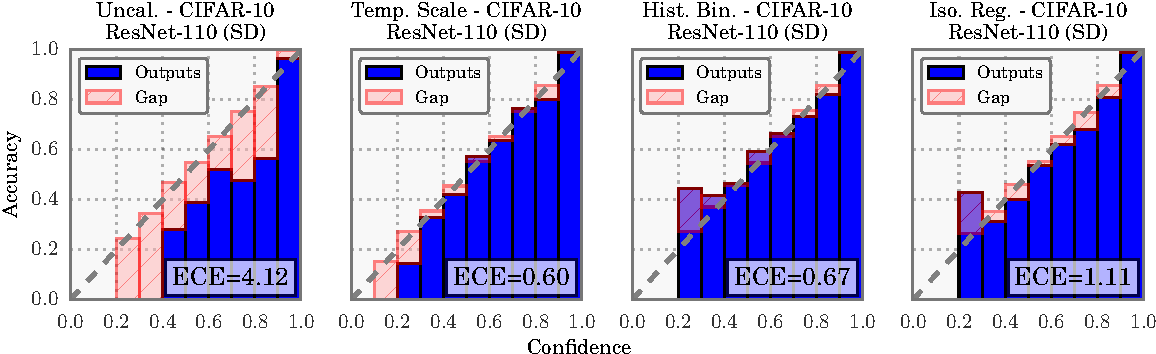
\includegraphics[width=\textwidth]{fig/reliability-cifar10.pdf}
  \caption{Reliability diagrams for CIFAR-10 before (far left) and after calibration (middle left, middle right, far right).}
  \label{figure.reliability-cifar10}
\end{figure*}
%
\begin{figure*}[h!]
  \centering
  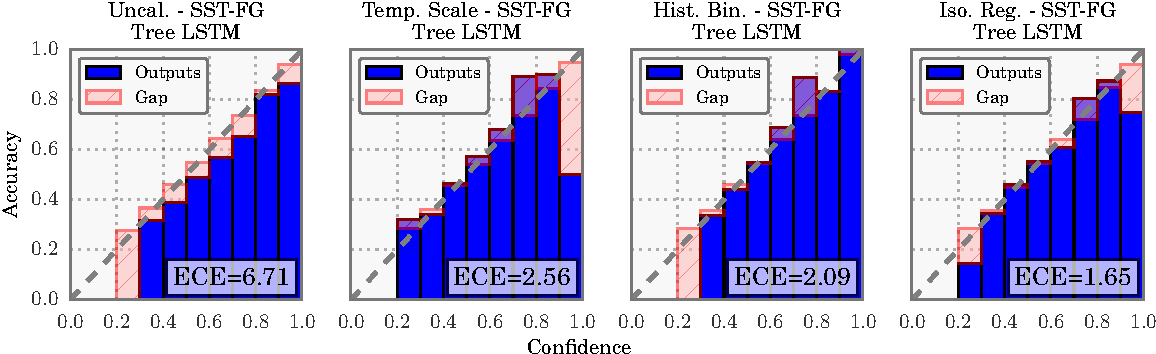
\includegraphics[width=\textwidth]{fig/reliability-SST_fine_grained.pdf}
  \caption{Reliability diagrams for SST Binary and SST Fine Grained before (far left) and after calibration (middle left, middle right, far right).}
  \label{figure.reliability-sst_fg}
\end{figure*}
\begin{figure*}[h!]
  \centering
  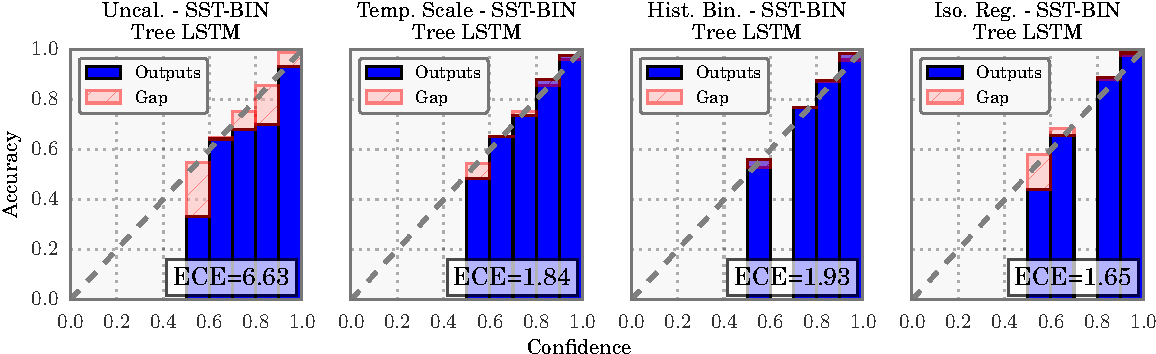
\includegraphics[width=\textwidth]{fig/reliability-SST_binary.pdf}
  \caption{Reliability diagrams for SST Binary and SST Fine Grained before (far left) and after calibration (middle left, middle right, far right).}
  \label{figure.reliability-sst_binary}
\end{figure*}

We include reliability diagrams for additional datasets: CIFAR-10 (\autoref{figure.reliability-cifar10}) and SST (\autoref{figure.reliability-sst_fg} and \autoref{figure.reliability-sst_binary}). Note that, as mentioned in \autoref{sec:definitions}, the reliability diagrams do not represent the proportion of predictions that belong to a given bin.
